% Time-stamp: <2022-11-07 05:29:09 A13258Q>
% Romain Lafarguette 2020, https://romainlafarguette.github.io/

%% ---------------------------------------------------------------------------
%% Preamble: Packages and Setup
%% ---------------------------------------------------------------------------
% Class 
\documentclass{beamer}

% Theme
\usetheme{Boadilla}
\usecolortheme{dolphin}
%\setbeamertemplate{headline}{} % Remove the top navigation bar

% Font and encoding
\usepackage[utf8]{inputenc} % Input font
\usepackage[T1]{fontenc} % Output font
\usepackage{lmodern} % Standard LateX font
\usefonttheme{serif} % Standard LateX font

% Maths 
\usepackage{amsfonts, amsmath, mathabx, bm, bbm} % Maths Fonts

% Graphics
\usepackage{graphicx} % Insert graphics
\usepackage{subfig} % Multiple figures in one graphic
\graphicspath{{/../static/img}{/../static/diagrams}}

% Layout
\usepackage{changepage}

% Colors
\usepackage{xcolor}
\definecolor{imfblue}{RGB}{0,76,151} % Official IMF color
\setbeamercolor{title}{fg=imfblue}
\setbeamercolor{frametitle}{fg=imfblue}
\setbeamercolor{structure}{fg=imfblue}

% Tables
\usepackage{booktabs,rotating,multirow} % Tabular rules and other macros
%\usepackage{pdflscape,afterpage} % Landscape mode and afterpage
%\usepackage{threeparttable} % Split long tables
\usepackage[font=scriptsize,labelfont=scriptsize,labelfont={color=imfblue}]{caption}

% Import files
\usepackage{import}

% Appendix slides
\usepackage{appendixnumberbeamer} % Manage page numbers for appendix slides

% References
\usepackage{hyperref}

% A few macros: environments
\newenvironment{wideitemize}{\itemize\addtolength{\itemsep}{10pt}}{\enditemize}
\newenvironment{wideenumerate}{\enumerate\addtolength{\itemsep}{10pt}}{\endenumerate}

\newenvironment{extrawideitemize}{\itemize\addtolength{\itemsep}{30pt}}{\enditemize}
\newenvironment{extrawideenumerate}{\enumerate\addtolength{\itemsep}{30pt}}{\endenumerate}

% Remove navigation symbols and other superfluous elements
\setbeamertemplate{navigation symbols}{}
\beamertemplatenavigationsymbolsempty

%\setbeamertemplate{note page}[plain]
\hypersetup{pdfpagemode=UseNone} % don't show bookmarks on initial view
\setbeameroption{hide notes}

% Institute font
\setbeamerfont{institute}{size=\footnotesize}
\DeclareMathSizes{10}{9}{7}{5}  

%% ---------------------------------------------------------------------------
%% Title info
%% ---------------------------------------------------------------------------
\title[Concepts]{Core Concepts in Financial Econometrics}
\author[R. Lafarguette]{Romain Lafarguette, Ph.D.}
\institute[IMF]{ADIA Quant \& IMF External Consultant\thanks{\scriptsize{\emph{This training material is the property of the International Monetary Fund (IMF) and is intended for use in IMF courses. Any reuse requires the permission of the IMF.}}}}

\date[STI, 08 Nov 2022]{Singapore Training Institute, 08 November 2022}

\titlegraphic{
    \begin{figure}
    \centering
    \subfloat{{
\includegraphics[width=2cm]{../static/img/imf_logo}}}%
    \end{figure}
}


% Slide between sections
\AtBeginSection[]
{
    \begin{frame}
        \frametitle{Table of Contents}
        \tableofcontents[currentsection]
    \end{frame}
}

%% ---------------------------------------------------------------------------
%% Title slide
%% ---------------------------------------------------------------------------
\begin{document}

\begin{frame}
\maketitle
\end{frame}


\begin{frame}{Outline of the Course}
\tableofcontents
\end{frame}


%% ---------------------------------------------------------------------------
%% Core
%% ---------------------------------------------------------------------------

\section{Data Concepts}

\begin{frame}
  \frametitle{Overview}

Financial econometrics (including time-series econometrics) are based on four main elements:\\
\smallskip

  \begin{wideenumerate}
    \item A sample of data
    \item An econometric model, based on a theory or not
    \item An estimation method to estimate the coefficients of the model
    \item Inference/testing approach to validate the estimation
  \end{wideenumerate}
  
\end{frame}


\begin{frame}
  \frametitle{Data Types}

  In econometrics, sets can be mainly distinguished in three types:\\
  \smallskip
  
  \begin{wideenumerate}
    \item Cross-sectional data
    \item Time series data
    \item Panel data
  \end{wideenumerate}
  
\end{frame}

% ADD some diagrams
\begin{frame}
  \frametitle{Cross-Sectional Data}
  Cross-sectional data are the most common type of data encountered in statistics and econometrics.\\ 
  \smallskip
  
  \begin{wideitemize}
    \item Data at the entities level: banks, countries, individuals, households, etc.
    \item \textbf{No time dimension}: only one "wave" or multiple waves of different entities
    \item Order of data does not matter: no time structure
  \end{wideitemize}
\end{frame}


\begin{frame}
  \frametitle{Time Series Data}

  Time series data are very common in financial econometrics and central banking. They entail specific estimation methods to do the \textbf{time-dependence}.\\

  \medskip
  
  \begin{wideitemize}
    \item Data for a single entity (person, bank, country, etc.) collected at multiple time periods. Repeated observations of the same variables (interest rate, GDP, prices, etc.)
    \item Order of data is important!
    \item The observations are typically not independent over time
  \end{wideitemize}  
\end{frame}


\begin{frame}
  \frametitle{Panel Data}
  Also called longitudinal data. They contain the most information and allow for more complex estimation and analysis.\\

  \medskip

  \begin{wideitemize}
    \item Data for multiple entities (individuals, firms, countries, banks, etc.) in which outcomes and characteristics of each entity are observed at multiple points in time
    \item Combine cross-sectional and time-series information
    \item Present several advantages with respect to cross-sectional and time series data, depending on the topic at hands
  \end{wideitemize}

\end{frame}


\begin{frame}
  \frametitle{Population vs. Sample}

  \begin{block}{Definition: Population}
    A \textbf{population} is defined as including all entities (e.g. banks or firms) or all the time periods of the processus that has to be explained
  \end{block}

\smallskip
  
  \begin{wideitemize}
    \item In most cases, it is impossible to observe the entire statistical population, due to constraints (recording period, cost, etc.)
    \item A researcher would instead observe a \textbf{statistical sample} from the population. He will estimate an econometric model to understand the \textbf{properties on the population as a whole}.
  \end{wideitemize} 
\end{frame}


\begin{frame}
  \frametitle{Data Generating Process}
  
  \begin{block}{Definition: Data Generating Process}
    \begin{itemize}
    \item A \textbf{Data Generating Process (DGP)} is a process in the real world that "generates" the data (or the sample) of interest.
    \item The process is represented by random variable (see after) $X_t$; the observation $x_t$ is one possible realization of $X_t$
    \item Given that we observe a set of $x_1, \dots, x_T$ what can we \textbf{infer} about the process $X_1, \dots, X_T$ that has generated them?
    \end{itemize}        
  \end{block}

  \begin{wideenumerate}
    \item The DGP is the "true" model that has generated the dataset $x_1, \dots, x_t$
    \item In reality, we can only observe the time series a \textbf{finite number of times}
    \item However, it is convenient to allow - theoretically - the number of observations to be \textbf{infinite}: $\{X_t\}_{t \ \in \ \mathbb{Z}}$. In this case,$\{X_t\}_{t \ \in \ \mathbb{Z}}$ is called a discrete time \textbf{stochastic process} 
  \end{wideenumerate}

  
\end{frame}

\begin{frame}

  \begin{exampleblock}{Example: Data Generating Process}
    Let us assume that there is a linear relationship between interest rates in two countries ($R, R^*$), their forward ($F$) and their spot exchange rate ($S$).\\

    \begin{equation*}
      \frac{F}{S} = \frac{1+R}{1+R^*}
    \end{equation*}

    This non-arbitrage relationship (CIP) can be used in the foreign exchange market to determine the forward exchange rate

    \begin{equation*}
      \mathbb{E}[F |S=s, R=r, R^*= r^*] = s*\frac{1+r}{1+r^*}
    \end{equation*}

This relationship is the \textbf{Data Generating Process} for $F$     
  \end{exampleblock}

The equivalent of population for time series econometrics is the DGP.\\
NB: note that I use $R$ to describe the random variable and $r$ to describe its realization
  
\end{frame}


\begin{frame}
  \frametitle{Econometrics Challenge}
  The challenge of econometrics is to draw conclusions about a DGP (or population), after observing only one realization $\{x_1, \dots X_N\}$ of a random sample (the dataset). To this end, we use a statistical - or econometrics - model\\

\medskip
  
    \makebox[\linewidth]{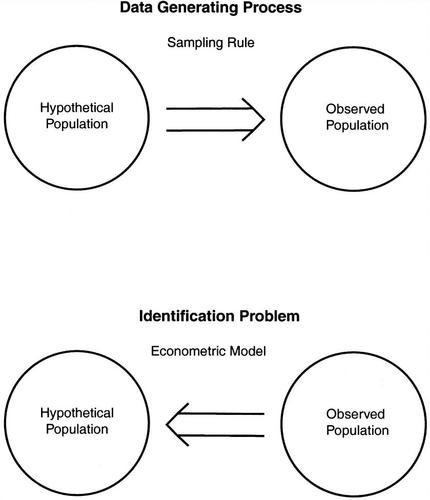
\includegraphics[height=0.6\paperheight]{../static/course_1_img/dgp_econometric_model.jpeg}}
  
  
\end{frame}


\section{Statistical Inference}

\begin{frame}
  \frametitle{Econometric Model}

  \begin{block}{Definition: Econometric Model}
    An econometric model specificies the statistical relationship between different economic variables, that are expected to be stable over time
  \end{block}

  \begin{enumerate}
  \item \textbf{Parametric model:} fully characterization of the relationship by a \textbf{set of parameters} $\theta$ and a \textbf{link function} $f$ supposed to be known; the specification can be linear or non linear, and includes some randomness $\epsilon$
    \begin{equation*}
      Y = f(X; \theta) + \epsilon
    \end{equation*}

  \item \textbf{Non-parametric and semi-parametric models}: the link function can not be described using a finite number of parameters. The link function is assumed to be unknown and has to be estimated
    
  \item The model is likely to be different from the DGP: there is a \textbf{model risk}
    
  \end{enumerate}
\end{frame}




\begin{frame}
  \frametitle{Example: A Linear Model}

  \begin{exampleblock}{Autoregressive Model: Look at the Past to Forecast the Future}
    A canonical basic time series model is the Autoregressive model of order $p$, called an AR model:

    \begin{equation*}
      X_t = \alpha_0 + \alpha_1 X_{t-1} + \alpha_2 X_{t-2} + \dots + \alpha_p X_{t-p} + \epsilon_t
    \end{equation*}       
  \end{exampleblock}

  \medskip

  \begin{itemize}
  \item $\epsilon_t$ is the randomness in the model: it represents a stochastic element that creates a discrepancy between the model and the reality. The role of a modeler is to reduce this discrepancy as much as possible
  \item The linear model is informative about the \textbf{conditional mean} of $X_t$, i.e. the average value of $X_t$ we can expect given certain past values $\tilde{X}_{t-1}$ of $X_t$
    \begin{equation*}
      \mathbb{E}[X_t|\tilde{X}_{t-1}, \tilde{X}_{t-2}, \dots, \tilde{X}_{t-p}] = \hat{\alpha}_0 + \hat{\alpha}_1 \tilde{X}_{t-1} + \hat{\alpha}_2 \tilde{X}_{t-2} + \dots + \hat{\alpha}_p \tilde{X}_{t-p}  
    \end{equation*}    
  \end{itemize}
  
\end{frame}


\begin{frame}
  \frametitle{How to Specify an Appropriate Time Series Model}
  \begin{wideenumerate}
    \item Study some \textbf{statistical properties} of the observed dat $\{x_t\}$, for instance, the \textbf{stationarity}, the patterns of the autocorrelation function \textbf{ACF}, or the \textbf{partial autocorrelation function}, etc.
    \item Compare these properties to the theoretical properties of some \textbf{typical time series models}, such as AR, MA, ARIMA, SARIMA, etc.
    \item Choose the most appropriate model and \textbf{estimate its parameters}
    \item Use this model for forecasting
  \end{wideenumerate}
\end{frame}


\begin{frame}
  \frametitle{Empirical Strategy}
  The general approach of (financial) econometrics is as follows:\\
  \smallskip

  \begin{wideenumerate}
  \item Specification of the model
  \item Estimation of the parameters
  \item Diagnostic tests
    \begin{itemize}
    \item Significance tests
    \item Specification tests
    \item Backtesting tests
    \item etc.
    \end{itemize}
  \item Interpretation and use of the model (forecasting, historical studies, etc.)
  \end{wideenumerate}
  
\end{frame}


\begin{frame}
  \frametitle{Refresher: Random Variables}
  \begin{wideitemize}
  \item Mathematicians are formalizing and modeling randomness via the concept of \textbf{random variables}.\\
  \item Pay attention: a random variable is neither random (it is formalized via laws and distributions), not a variable (it is a function)
  \item A \textbf{random variable} is a function $f: \Omega \mapsto \mathcal{R}$ that assigns to
      a set of outcome $\Omega$ a \textbf{value}, often a real number.
  \item The probability of an outcome is equal to its \textbf{measure} divided by
        the measure of all possible outcomes
     \begin{itemize}
      \item Example: obtaining an even number by rolling a dice: $\{2, 4, 6\}$
      \item Probability to obtain an even number by rolling a dice: $m(\{2, 4,
        6\})/m(\{1, 2, 3, 4, 5, 6\}) = \frac{1}{2}$ \emph{(here, the measure
          simply "counts" the outcomes with equal weights)}
        \end{itemize}     
  \end{wideitemize}  
\end{frame}

\begin{frame}
  \frametitle{Random Variables (II)}    
  \begin{itemize}
  \item Random variables are the "building block" of statistics:
    \begin{wideitemize}
    \item Random variables are characterized by their distribution (generating
      function, moments, quantiles, etc.)
    \item The behavior of two or more random variables can be characterized by
      their dependence/independence, matrix of variance-covariance, joint
      distribution, etc.
    \item The main theorems in statistics (law of large numbers, central limit
      theorem, etc.) leverage the properties of random variables
    \end{itemize}
  \end{wideitemize}
\end{frame}


\begin{frame}
  \frametitle{Refresher: Probability Distributions for Continuous Variables}
  
  \begin{block}{Definition: Probability Distribution}
    The probability distribution of a random variable describes how the probabilities of the outcomes are distributed. How more likely is one outcome compared to another? Is there more upside risk or downside risk? Etc.
  \end{block}

\medskip
  
  Distributions are equivalently represented by their:
  \begin{enumerate}
  \item \textbf{The probability density function (pdf)}
  \item \textbf{The cumulative distribution function (cdf)}  
  \end{enumerate}    
  
  The pdf is also necessary to define distributions' moments (see after).\\  
\end{frame}
  
\begin{frame}
  \begin{wideitemize}
  \item \textbf{The probability density function (pdf)} usually denoted $f_X(x0)$ (remember than $X$ stands for the random variable, while $x0$ stands for a realization of the random variable) represents the relatively likelihood that the random variable $X$ will fall within a small neighborhood of $x0$ (infinitesimal concept). It is easier to conceptualize the pdf via the cdf
  \item \textbf{The cumulative distribution function (cdf)} usually denoted $F_X(x0)$ represents the probability that the random variable will be lower than $x0$. It cumulates the pdf ("all the small neighborhoods") such that:
    \begin{equation*}
F_X(x0) \equiv \mathbb{P}[X \leq x0] = \int_{-infty}^{x0} f_X(h) dh      
    \end{equation*}    
  \end{wideitemize}  
\end{frame}


\begin{frame}
\frametitle{Link between PDF and CDF}
    \makebox[\linewidth]{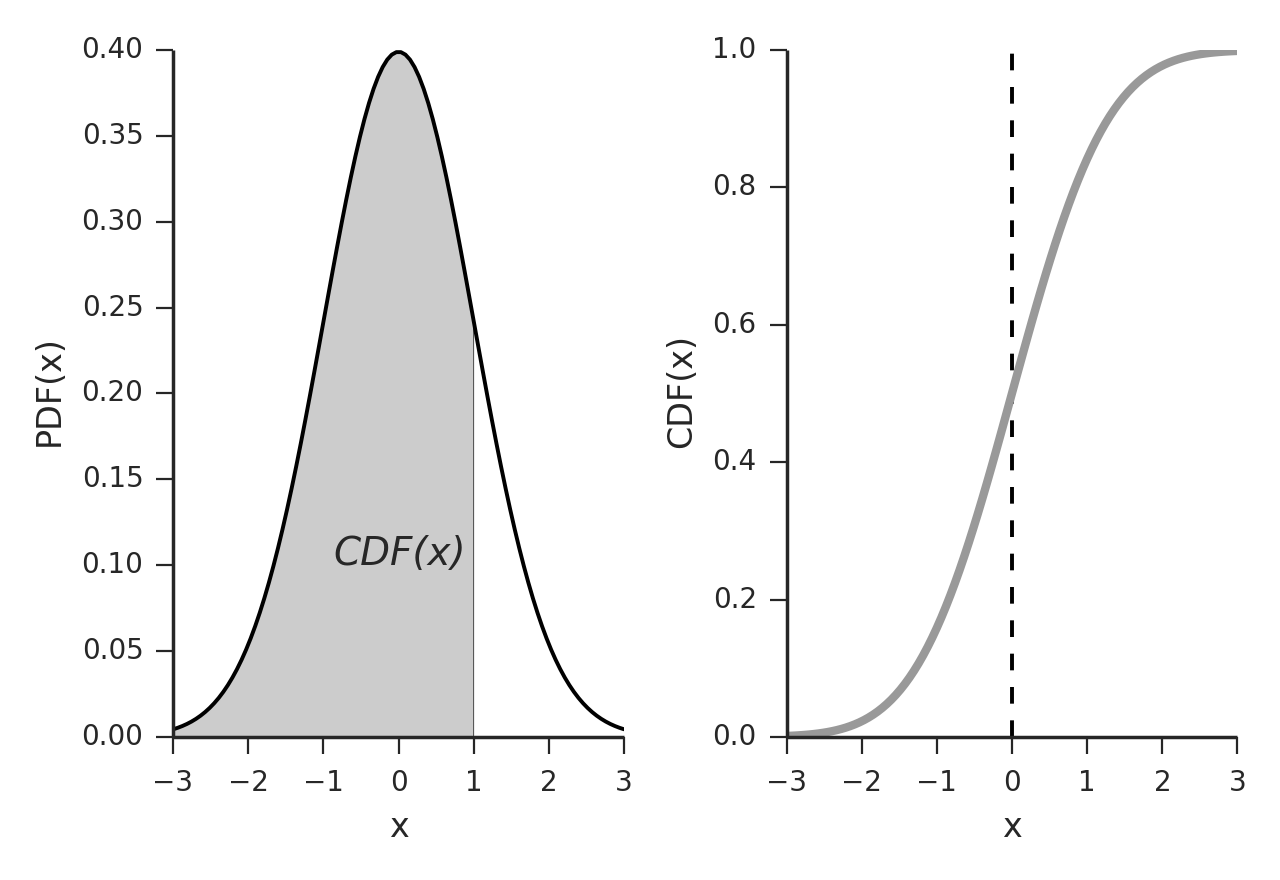
\includegraphics[width=0.85\paperwidth]{../static/course_1_img/pdf and cdf.png}}
\end{frame}


\begin{frame}
  \frametitle{Moments: Overview}
  \begin{table}
    \centering
    \begin{tabular}{lll}
      \hline
      \hline
      & Formula & Interpretation \\
      \hline
      \textbf{Mean} & $\mathbb{E}[X_t] = \mu$ & Central tendency\\
      \textbf{Variance} & $\mathbb{V}[X] = \mathbb{E}\left[(X_t - \mu)^2\right] = \sigma^2$ & Dispersion around $\mu$\\
      \textbf{Skewness} & $\mathbb{S}[X] = \mathbb{E}\left[(X_t - \mu)^3\right] = \text{sk}$ & Symmetry\\
      \textbf{Kurtosis} & $\mathbb{K}[X] = \mathbb{E}\left[(X_t - \mu)^4\right] = \kappa$ & Tail heaviness\\
      \hline
      \hline                                                                                            
    \end{tabular}
  \end{table}
\end{frame}


% TODO: add charts

\begin{frame}
  \frametitle{Moments: In Practice}

  \begin{wideitemize}
    \item The moments allow to characterize the shape of the returns distribution
    \item However, the theoretical moments are \textbf{unobservable} and need to be estimated
    \item Assume that we have a sample $\{x_1, \dots, x_T\}$ realizations of the sequence of $X_t$
  \end{wideitemize}
  
\end{frame}



\begin{frame}
  \frametitle{Estimator}

  \begin{block}{Definition: Estimator}
    An \textbf{estimator} is any function $F(x1, \dots, x_t)$ of a sample. Note that any descriptive statistics is an estimator (a simple one) 
  \end{block}


  \begin{exampleblock}{Example: Sample Mean}
    The sample mean (or overage) of a sample is an estimator of the (theoretical) mean $ \mathbb{E}[X_t] = \mu$.\\
    The estimator is simply: $\hat{\mu_t} \equiv \bar{X_t} = \frac{1}{T} \sum_{t=1}^{T}x_t$
  \end{exampleblock}
  
\end{frame}


\begin{frame}
  \frametitle{Example: Variance}

  \begin{exampleblock}{Example: Sample Mean}
    Assume that the observations are drawn from \emph{i.i.d} random variables.\\
    The \textbf{sample variance} $\hat{sigma}^2_T = \frac{1}{T-1} \sum_{t=1}^T (x_t - \bar{x}_t)^2$
  \end{exampleblock}

\textbf{Note:} the denominator is equal to \emph{T-1} as to define a sample variance corrected for the small sample bias. 
  
\end{frame}



\begin{frame}
  \frametitle{Sampling Distribution}

  \begin{block}{Fact}
    An estimator $\hat{\theta}$ is a \textbf{random variable}
  \end{block}
  Therefore, $\hat{\theta}$ has a (marginal or conditional) \textbf{probability distribution}. This sampling distribution is characterized by a probability distribution function (pdf) $f_{\hat{\theta}}(u)$

  \begin{block}{Definition: Sampling Distributions}
    The probability distribution of an estimator is called the \textbf{sampling distribution}
  \end{block}
  The sampling distribution is described by its moments, such as expectations, variance, skewness, etc.
  \end{frame}


  \begin{frame}
    \frametitle{Point Estimate}
    \begin{block}{Definition: Estimate}
      An estimate is the realized value of an estimator (e.g. a number, in a case of a point estimate) that is obtained for a particular value $x0$. Often noted as $\hat{\theta}(x0)$ for the estimator $\hat{\theta}$
    \end{block}

    \begin{exampleblock}{Estimate of a linear regression}
      \begin{itemize}
      \item DGP $Y = \alpha + \beta*X + \epsilon$, with joint sample ${y1, \dots, y_T}, {x1, \dots, x_T}$.\\
      \item We have an estimator (for instance an OLS) of $\hat{\alpha}, \hat{\beta}$
      \item Then, for any value of $X=x_0$, we can simply project the \textbf{conditional expected estimate} $y_0 = \hat{\alpha} + \hat{\beta}*x_o + \hat{\epsilon}$
      \item If the estimator is unbiased, the fitted residuals $\hat{\epsilon} = y_t - \hat{\alpha} - \hat{\beta}*x_t$ are centered on \textbf{average}:$\mathbb{E}\left[\hat{\epsilon}\right]=0$. This is why the residual disappear from the estimate of the conditional expected estimate in an OLS... but no bias doesn't mean no variance !
      \item $\epsilon$ \& $\hat{\epsilon}$ are random variables: they determine $\hat{\alpha}, \hat{\beta}$ distributions
      \end{itemize}
    \end{exampleblock}    
  \end{frame}


  \begin{frame}
    \frametitle{What Constitutes a Good Estimator?}
    The idea is to study the properties of the \textbf{sampling distribution} of the estimator $\hat{\theta}$, and especially its moments, such as:\\

    \medskip

    \begin{wideitemize}
    \item $\mathbb{E}[\hat{\theta}]$ for the biais
    \item $\mathbb{V}[\hat{\theta}]$ for the precision
    \item $\mathbb{S}[\hat{\theta}]$ for the symmetry
    \item $\mathbb{K}[\hat{\theta}]$ for the tail-risks  
    \item etc.
    \end{wideitemize}
  \end{frame}


  \begin{frame}
    \frametitle{Estimators Properties}
    Estimators are compared on the basis of a variety of attributes

    \begin{wideenumerate}
      \item \textbf{Finite sample properties} (or finite sample distributions) investigate how the estimator behave when the observational sample is relatively limited (a few hundreds to a few thousands of observations max)
      \item However, these properties rely on a distributional assumption (usually normality or gaussianity), that may be difficult to test. 
      \item When the normality assumption is no longer valid (and the finite sample distribution is unknown), estimators are evaluated on the basis on their \textbf{large sample}, or \textbf{asymptotic properties}
    \end{wideenumerate}    
  \end{frame}


  \begin{frame}
    \frametitle{Finite Sample Theorem}
    \begin{block}{Theorem: Finite Sample Distributions}
        If we assume that, with a sample of size $T$, generated from a stochastic process with i.i.d random variables $X_1, X_2, \dots, X_T$  with $X_{t} \sim \mathcal{N}(\mu, \sigma^2)$, then the estimators of the sample mean $\hat{\mu_T}$ and the estimator of the sample variance/population variance $(T-1) \frac{\hat{\sigma^2_T}}{\sigma^2}$ have a \textbf{finite sample distribution}

        \begin{equation*}
          \hat{\mu_T} = \mathcal{N}\left(\mu, \frac{\sigma^2}{T} \right) \qquad \forall \ T \ \in \ \mathbb{N}
        \end{equation*}


        \begin{equation*}
          \frac{T-1}{\sigma^2} \hat{\sigma^2} \sim \chi^{2} (T-1) \qquad \forall T \ \geq \ 2
        \end{equation*}
        
      \end{block}
\end{frame}


\begin{frame}
      \begin{exampleblock}{Example: Finite Sample Distribution}
        Under the Gaussianity assumption, with a sample size of $T = 10$, then:
        \begin{equation*}
          \hat{\mu} \sim \mathcal{N}\left( \mu, \frac{\sigma^2}{10} \right) \qquad 9 \times \frac{\hat{sigma^2_T}}{\sigma^2} \sim \chi^2(9)
        \end{equation*}        
      \end{exampleblock}
      
  \end{frame}
  

  \begin{frame}
    \frametitle{Difficulties with Finite Sample Inference}
    In most cases, it is impossible to derive the \textbf{exact/finite sample distribution} for the estimator (or any transformation of the estimator).

    \begin{wideenumerate}
    \item In some cases, the exact distribution of $\{ X1, X2, \dots, X_T\}$ is known, but the estimator function $S()$ (also called the "statistics") is too complicated
      \begin{equation*}
        \hat{\theta} = S(X_1, X_2, \dots, X_T) \sim ??? \qquad \forall \ T \ \in \mathbb{N}
      \end{equation*}

      \item In most cases, the distribution of the stochastic process $\{X1, X2, \dots, X_T\}$ is unknown

      \begin{equation*}
        \hat{\theta} = S(X_1, X_2, \dots, X_T) \sim ??? \qquad \forall \ T \ \in \mathbb{N}
      \end{equation*}        
    \end{wideenumerate}
    
  \end{frame}
  


  \begin{frame}
    \frametitle{Asymptotic Properties}

    What is the behavior of the estimator $\hat{\theta_T}$ when the sample size $T$ tends to infinity?

    \begin{block}{Definition: Asymptotic Theory}
      \textbf{Asymptotic} or \textbf{large sample theory} consists in the study of the distribution of the estimator when the sample size is sufficiently large (usually, more than 10k)
    \end{block}

    The asymptotic theory is fundamentally based on the notion of \textbf{convergence}
    
  \end{frame}
  

  \begin{frame}
    \frametitle{Convergence in Probability}
    There are many types of convergence, but typically applied statisticians are interested in:
   
    \begin{enumerate}
      \item Convergence in probability
      \item Convergence in distribution
    \end{enumerate}

    \begin{itemize}
\item  \textbf{Convergence in probability} (also called "mean squared convergence" or "almost sure convergence")

  \begin{equation*}
    \hat{\theta_T} \ \overset{p}{\to} \ \theta \qquad \text{for} \ \theta \ \in \ \mathbb{R}
  \end{equation*}

\item Technically, for a stochastic process ${\theta_T}_{-\infty}^ {+\infty}$
  \begin{equation*}
  \hat{\theta_T} \ \overset{p}{\to} \theta \quad \Leftrightarrow \quad \text{lim}_{T \to +\infty} \mathbb{P} \left[ |\theta_T - \theta| > \epsilon \right] \ = \ 0 
  \end{equation*}
    
\item The convergence in probability is used to derive the \textbf{consistency property} of estimators
    \end{itemize}
    
  \end{frame}


  \begin{frame}
    \frametitle{Illustration: Distribution in Probability}
    
    \begin{equation*}
\hat{X_T} \ \overset{p}{\to} c \ \text{if} \ \Leftrightarrow \quad \text{lim}_{T \to +\infty} \mathbb{P} \left[ |X_T - c| > \epsilon \right] \ = \ 0      
    \end{equation*}

    
     \makebox[\linewidth]{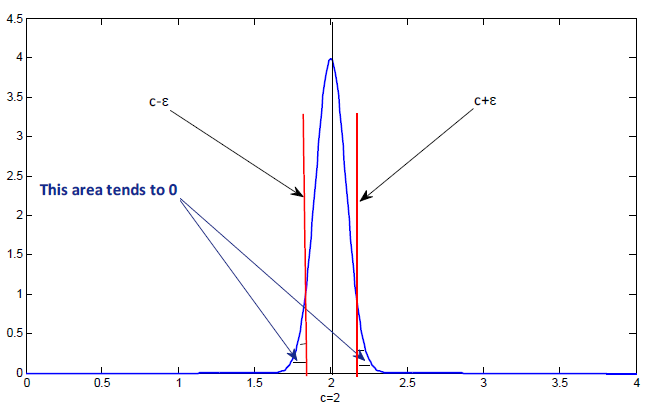
\includegraphics[width=0.7\paperwidth]{../static/course_1_img/distribution_in_proba.PNG}}
    
  \end{frame}


  \begin{frame}
    \frametitle{Interpretation}
    \begin{wideenumerate}
    \item The distribution of the sample moments is highly concentrated around the true value (unknown) of the population moment when the sample size $T$ tends to infinity
    \item In other words, over a very large sample of data (for instance, hundred of thousands of observations) the \textbf{moments estimated in the sample} are then very "close" to the true value of \textbf{the moments in the population}
    \end{wideenumerate}
  \end{frame}
  

  \begin{frame}
    \frametitle{Convergence in Distribution}

    \begin{itemize}
\item  \textbf{Convergence in distribution} is interested in the distribution of the bias (the distance between the estimator and the true value)

  \begin{equation*}
    \sqrt{T} \left(\hat{\theta_T} - \theta_0 \right) \ \sim \ \mathcal{N}(\mu_., \sigma_.) \qquad \mathcal{N} \ \text{is the most common} 
  \end{equation*}

\item Technically, for a stochastic process ${X_T}_{-\infty}^ {+\infty}$, with a cdf $F_T(.)$; $X_T$ is said to \textbf{converge in distribution} to a random variable $X$ if:
  \begin{equation*}
X_t \ \overset{d}{\to} \ X \quad \Leftrightarrow \quad  F_T(x) = F(x) \qquad \ \forall \ x \ \in \ \mathbb{R}
  \end{equation*}
    
\item The convergence in distribution is used to derive the \textbf{asymptotic distribution} of the estimators and to make \textbf{inference} (tests) about the true value of the parameters

    \end{itemize}
    
  \end{frame}



\section{Statistical Features and Properties}

\begin{frame}
  \frametitle{Stylized Properties}

  Fan and Yao (2015, the Elements of Financial Econometrics) identify 8 main "stylized facts"
  
  \begin{enumerate}
  \item Stationarity
  \item Absence of autocorrelations
  \item Heavy tails
  \item Asymmetry
  \item Volatility clustering
  \item Aggregational Gaussianity
  \item Long range dependence
  \item Leverage effect
  \end{enumerate}
  
\end{frame}



\begin{frame}
  \frametitle{Stationarity}
  \begin{exampleblock}{Example}
   In general, prices are non-stationary but returns are stationary 
 \end{exampleblock}

 \begin{block}{Definition: Weak Stationarity (Second Order Stationarity)}
   A stochastic process ${X_t}_{t \in \mathbb{Z}}$ is weakly stationary if and only if:

   \begin{itemize}
   \item $\mathbb{E}(X^2_t) \ < \ \infty \ \quad \forall \ t \ \in \ \mathbb{Z}$
   \item $\mathbb{E}(X_t) = \mu \ \quad \forall \ t \ \in \ \mathbb{Z}$ doesn't depend on $t$
   \item $\text{Cov}(x_t, x_{t+h}) \ = \ \mathbb{E}[(x_{t+h} - m)(x_t - m)] \ = \ \gamma_h \quad \forall \ (t, h) \ \in \ \mathbb{Z}^2$ desn't depend on $t$
   \end{itemize}
   
 \end{block}
 
\end{frame}


\begin{frame}
  \frametitle{Intuitive Interpretation}
   Weak stationarity means that the stochastic process oscillates around a constant level, is not trended and has the following properties:\\
  
  \begin{wideenumerate}
  \item The mean and time-covariance are constant over time
    \begin{equation*}
\mathbb{E}(X_t) = \mu \qquad \mathbb{C}ov(X_t, X_{t-h}) = \gamma(h) \qquad \forall \ h \ \in \ \mathbb{Z}
\end{equation*}
\item Because the time-covariance is constant over time, it implies that the variance is also constant over time
  \begin{equation*}
\mathbb{V}(X_t) = \mathbb{C}ov(X_t, X_{t-h}) = \gamma(0) \qquad \forall \ t \ \in \ \mathbb{Z}
  \end{equation*}
\item $\mathbb{C}ov(X_t, X_{t-h}) = \gamma(h) \qquad \forall \ h \ \in \ \mathbb{Z}$ can be interpreted as "\emph{covariance doesn't change when shifted in time}"
  \begin{equation*}
\mathbb{C}ov(X_r, X_s) = \mathbb{C}ov(X_{r+t}, X_{s+t}) \qquad \forall \ (r, s, t) \ \in \ \mathbb{Z}^3
  \end{equation*}
  
  \end{wideenumerate}
\end{frame}


\begin{frame}
\frametitle{Prices are Usually Non-Stationary...}
    \makebox[\linewidth]{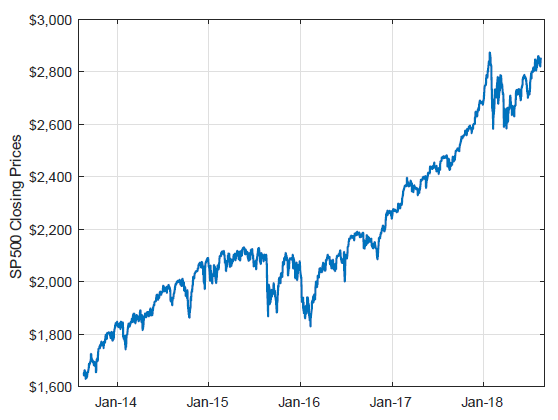
\includegraphics[width=0.7\paperwidth]{../static/course_1_img/non stationarity prices sp500.PNG}}
\end{frame}


\begin{frame}
\frametitle{... But Returns Are !}
    \makebox[\linewidth]{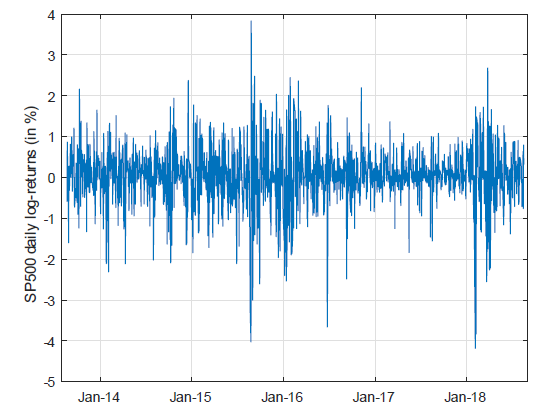
\includegraphics[width=0.7\paperwidth]{../static/course_1_img/stationarity returns sp500.PNG}}
\end{frame}


\begin{frame}
  \frametitle{Absence of autocorrelations}
  \begin{exampleblock}{Fact: Common absence of autocorrelations}
    The autocorrelations of assets returns (in general) are often insignificant, except for very small intraday time scales (around 20 minutes) for which the microstructure effects come into play
  \end{exampleblock}

\textbf{Note:} The fact that returns hardly show any serial correlation does not mean that they are independent


\begin{block}{Definition: Autocorrelation}
  The autocorrelation, denoted $\rho(k)$ of a weak stationary process $X_t$ is the correlation between the values of the process at different times:

  \begin{equation*}
    \rho_k \ = \ \text{Corr}(X_t, X_{t-k}) \ = \ \frac{\mathbb{E}\left[ (X_t - \mu)(X_{t-k} - \mu)\right]}{\mathbb{V}(X_t)} = \frac{\gamma_k}{\sigma^2}
  \end{equation*}

with $\mu = \mathbb{E}[X_t]$, $\sigma^2 = \mathbb{V}(X_t), \ \forall \ t$ and $\gamma_k$ the autocovariance of order $k$
  
\end{block}

\end{frame}

\begin{frame}
  \frametitle{Measuring Sample Autocorrelation}
  \begin{block}{Definition: Sample Autocorrelation}
    The \textbf{sample autocorrelation}, denoted $\hat{\rho}(k)$ of a weak stationary process $X$ is an estimator of $\rho(k)$ defined as:

    \begin{equation*} 
      \hat{\rho}_k = \text{corr}(X_t, X_{t-k}) = \frac{1}{(T-k)\hat{\sigma^2}} \sum_{t=k+1}^{R}(X_t - \hat{mu})(X_{t-k} - \hat{mu})
    \end{equation*}
where $\hat{\sigma^2}$ and $\hat{\mu}$ are consistent estimators of $\mu = \mathbb{E}(X_t)$ and $\sigma^2 = \mathbb{V}(X_t) \qquad \forall t$
  \end{block}
\end{frame}


\begin{frame}
  \frametitle{Example: Autocorrelation of the SP500}
  The \textbf{Autocorrelation Function (ACF)} (or \textbf{correlogram}) represents the sample autocorrelation for different lags, from $k=1$ to a maximum lag order, for instance $k=15$

 \makebox[\linewidth]{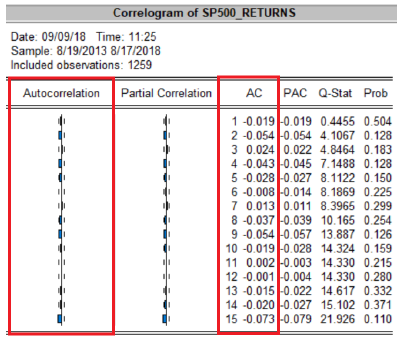
\includegraphics[width=0.5\paperwidth]{../static/course_1_img/autocorrelogram.PNG}}
  
\end{frame}



\begin{frame}
  \frametitle{Asymmetry}

  \begin{block}{Stylized Fact: Heavy Tails}
    The distribution of many financial variables, including asset returns, are often \textbf{asymmetric} and \textbf{negatively skewed}
  \end{block}

  \begin{itemize}
  \item Asymmetry is defined by the skewness, which is the third-order moment (see before)
  \item This reflects the fact that the downturns of financial markets are often much steeper than the recoveries
  \item Investors tend to react more strongly to negative news that to positive news 
  \end{itemize}
\end{frame}


\begin{frame}
  \frametitle{Skewness}
  There are different shapes of kurtosis 
 \makebox[\linewidth]{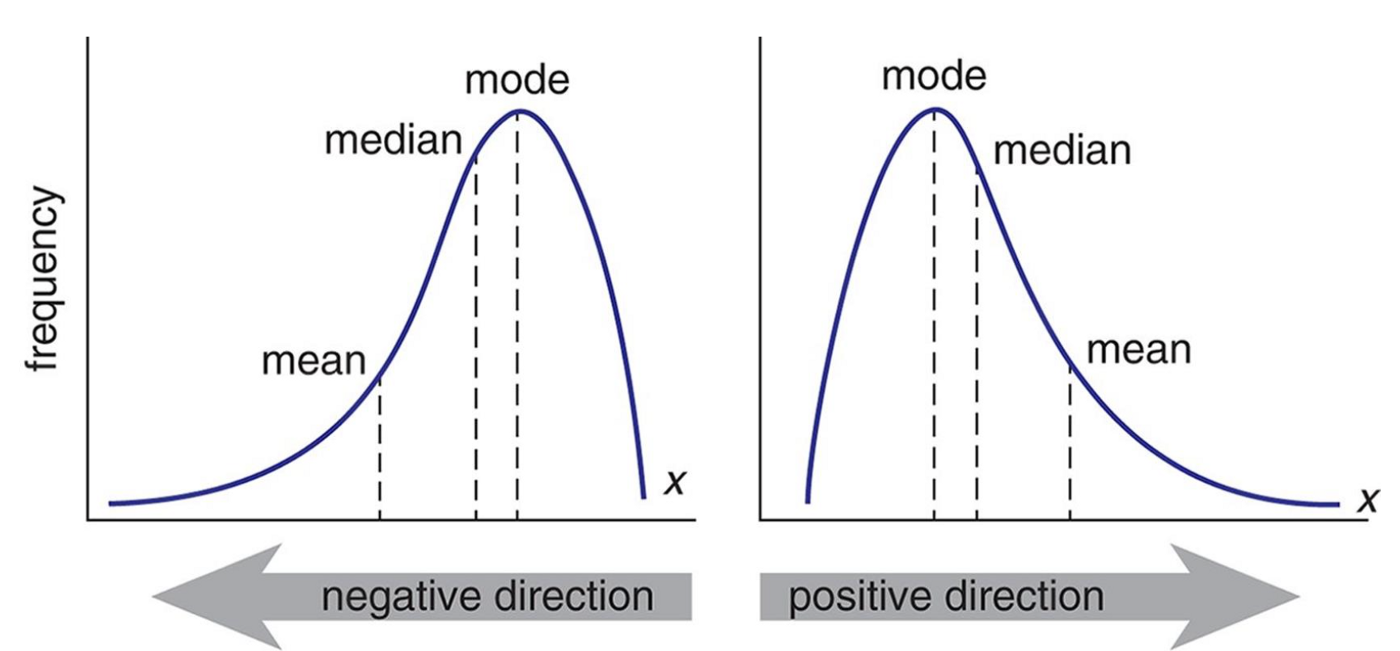
\includegraphics[width=0.8\paperwidth]{../static/course_1_img/skewness.PNG}}  
\end{frame}



\begin{frame}
  \frametitle{Heavy Tails}
  \begin{exampleblock}{Fact: Heavy Tails}
    The probability distribution of many financial variables, including asset returns, often exhibit \textbf{heavier tails} than those of a normal distribution
  \end{exampleblock}

  \begin{itemize}
  \item "Heavier tails" are rigorously defined by the kurtosis, which is the fourth-order moment (see before)
  \item Mandelbrot (1963) recognized the heavy-tailed, highly peaked nature of certain financial time series
  \item These heavy tails can be explained by risk aversion, heard behavior, market microstructure (illiquidity, asymmetric information, etc.)
  \end{itemize}    
\end{frame}



\begin{frame}
  \frametitle{Normal versus Tails}
  There are different shapes of kurtosis 

 \makebox[\linewidth]{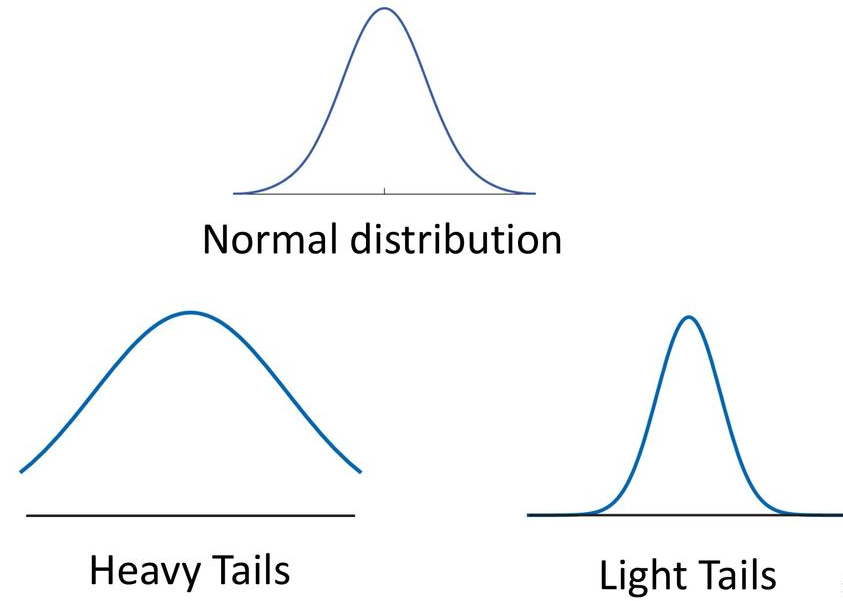
\includegraphics[width=0.8\paperwidth]{../static/course_1_img/normal versus tails.PNG}}  
\end{frame}


\begin{frame}
  \frametitle{Forms of Kurtosis (Fat Tails)}
  There are different shapes of kurtosis:\\ 
 \makebox[\linewidth]{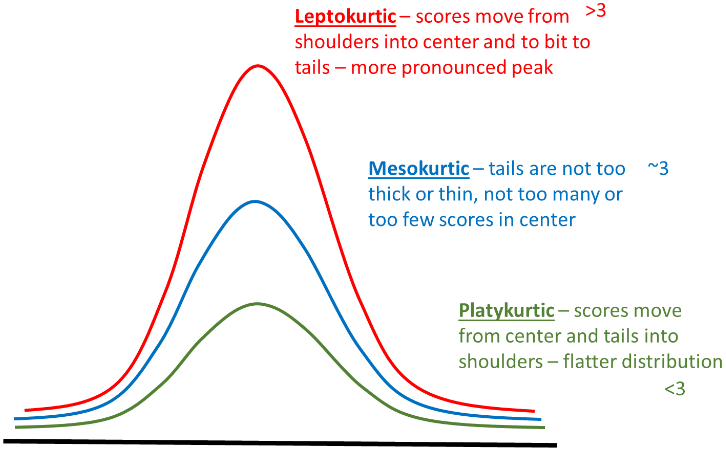
\includegraphics[width=0.8\paperwidth]{../static/course_1_img/forms of kurtosis.PNG}}  
\end{frame}


\begin{frame}
  \frametitle{Volatility Clustering}
  \begin{block}{Definition: Volatility Clustering}
    \begin{itemize}
    \item \textbf{Volatility clustering} means that large price changes (i.e. returns with large absolute values or large squares) occur in clusters
    \item Large price changes tend to be followed by large price changes (up and down)
    \item Periods of tranquility alternate with periods of high volatility (volatility regimes)
    \end{itemize}
    
    \emph{Note: volatility clustering is the consequence of the autocorrelation of the squared returns}\\
    
  \end{block}
\end{frame}


\begin{frame}
  \frametitle{Volatility Regimes: US VIX}
  The VIX is the implied volatility fo the US SP 500:\\ 
 \makebox[\linewidth]{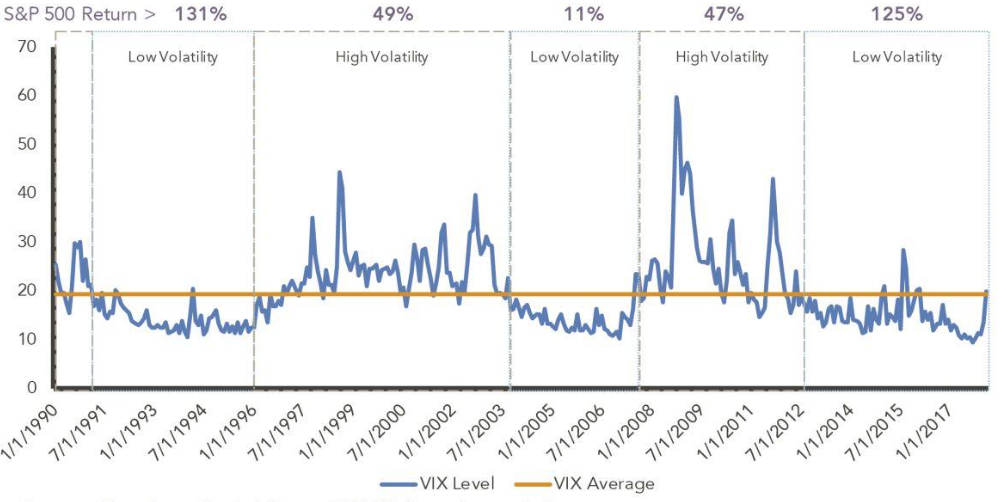
\includegraphics[width=0.8\paperwidth]{../static/course_1_img/vix volatility.PNG}}  
\end{frame}


\begin{frame}
  \frametitle{Aggregational Gaussianity}

  \begin{block}{Definition: Aggregational Gaussianity}
    \begin{itemize}
    \item Asset returns over $k$ days is simply the aggregation of $k$ daily returns
    \item When the time horizon $k$ increases, the central limit theory says that the distribution of returns over a long-time horizon (a few months) tends toward a \textbf{normal distribution}
    \end{itemize}
  \end{block}


  \begin{itemize}
  \item Aggregational gaussianity implies that over long horizons, the pecularities of financial time series over short-term horizon (skewness, kurtosis, etc.) tend to vanish
  \item However, in finance, people are mostly interested in relatively short-term movements, suggesting that working under the gaussianity assumption is often not appropriate
  \end{itemize}
  
\end{frame}


\begin{frame}
  \frametitle{Aggregational Gaussanity In Practice}
  The VIX is the implied volatility fo the US SP 500:\\ 
 \makebox[\linewidth]{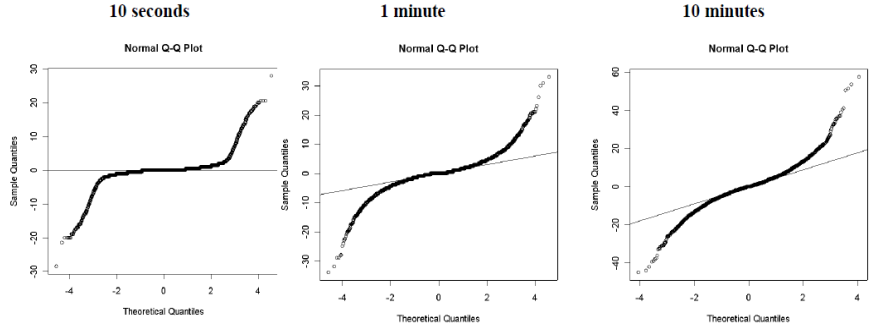
\includegraphics[width=0.8\paperwidth]{../static/course_1_img/aggregational gaussianity.PNG}}  
\end{frame}


\begin{frame}
  \frametitle{Long Range Dependence}
  \begin{block}{Definition}
    \begin{itemize}
    \item At the difference of log returns or standard returns, daily squared returns and absolute returns often exhibit significant autocorrelations
    \item Those autocorrelations are persistent, indicating possible \textbf{long-memory} properties
    \end{itemize}
  \end{block}

\emph{Those autocorrelations become weaker and less persistent when the sampling interval is increased to a week or a month}\\
  
\end{frame}


\begin{frame}
  \frametitle{Long Range Dependence}
  SP 500 Returns (left) and squared returns (right) \\

\medskip
  
 \makebox[\linewidth]{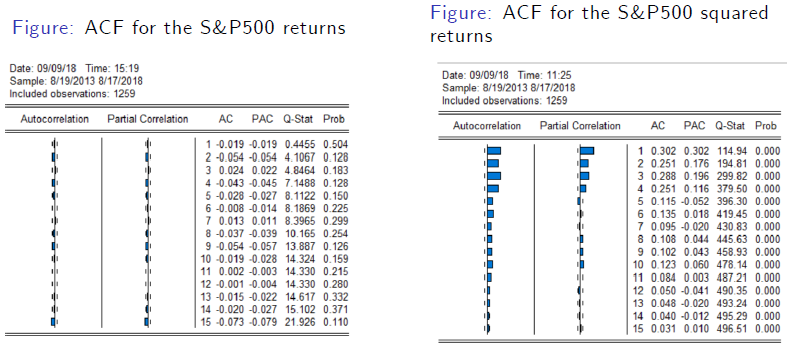
\includegraphics[width=0.8\paperwidth]{../static/course_1_img/long range dependence.PNG}}  
\end{frame}



\begin{frame}
  \frametitle{The ARCH effect}
  \begin{itemize}
  \item The autocorrelation of the squared returns is called the \textbf{ARCH effect} (auto-regressive conditional heteroskedasticity)
  \item It is most important with daily returns, and less important with low frequency returns (monthly, quarterly, etc.)
  \end{itemize}

\medskip
  
ARCH effect is important in finance, because it describes patterns on the dynamic of financial volatility 
  
\end{frame}



\begin{frame}
  \frametitle{Leverage Effect}

  \begin{block}{Definition: the Leverage Effect}
    \begin{itemize}
    \item Assets returns are negatively correlated with the changes in their volatilities
    \item This negative correlation $\text{Corr (returns, vol)}$ is called the \textbf{leverage effect}
    \end{itemize}

Financial explanations
    \begin{itemize}
    \item An asset price declines, companies mechanically become more leveraged (debt-to-equity ratio up) and riskier: therefore, their stock prices become more volatile
    \item On the other hand, when stock prices become more volatile, investors demand high returns and hence stock prices go down
    \item Volatilities caused by price decline are typically larger than prices appreciation due to declined volatilities
    \end{itemize}
    
  \end{block}
  
\end{frame}





\end{document}












\section{Misc}

\begin{frame}
  \frametitle{Stochastic Process}

  \begin{itemize}
  \item A stochastic process is a sequence of random variables indexed by time
    ($t$):
    \begin{equation*}
      {\dots, Y_1, Y_2, \dots, Y_t, Y_{t+1}, \dots} = 
    \end{equation*}
    
  \end{itemize}
  

  
\end{frame}


\begin{frame}
  \frametitle{Ergodicity}
  
\end{frame}


\begin{frame}
  \frametitle{Biais Variance Tradeoff}
  
\end{frame}


\begin{frame}
  \frametitle{Efficiency}
  
\end{frame}


\begin{frame}
  \frametitle{Simson Paradox}
  
\end{frame}






%% ---------------------------------------------------------------------------
%% End document
%% ---------------------------------------------------------------------------
\end{document}


%% ---------------------------------------------------------------------------
%% Sample code
%% ---------------------------------------------------------------------------

% \begin{frame}
% \frametitle{Example with a Figure}
%     \makebox[\linewidth]{\includegraphics[width=\paperwidth]{../output/step_007_top_ae_dotplot.pdf}}
% \end{frame}


% \begin{frame}
% \begin{adjustwidth}{-2em}{-2em} % Wider frame 
%   \frametitle{Example with a Wide Table}  
%   \setlength\tabcolsep{4pt}  % default value: 6pt
%   %\footnotesize
%   \centering
%   \input{../output/mytable.tex}\\
% \end{adjustwidth}
% \end{frame}









%%% Local Variables:
%%% mode: latex
%%% TeX-master: t
%%% End:
